
% Define listing style for yaml
\newcommand\YAMLcolonstyle{\color{black}\bfseries\small}
\newcommand\YAMLkeystyle{\color{black}\mdseries\small}
\newcommand\YAMLvaluestyle{\color{green}\mdseries\small}

\makeatletter

% here is a macro expanding to the name of the language
% (handy if you decide to change it further down the road)
\newcommand\language@yaml{yaml}

\expandafter\expandafter\expandafter\lstdefinelanguage
\expandafter{\language@yaml}
{
  keywords={true,false,null,y,n},
  keywordstyle=\color{darkgray}\bfseries,
  basicstyle=\YAMLkeystyle,                                 % assuming a key comes first
  sensitive=false,
  comment=[l]{\#},
  morecomment=[s]{/*}{*/},
  commentstyle=\color{purple}\ttfamily,
  stringstyle=\YAMLvaluestyle\ttfamily,
  moredelim=[l][\color{orange}]{\&},
  moredelim=[l][\color{magenta}]{*},
  moredelim=**[il][\YAMLcolonstyle{:}\YAMLvaluestyle]{:},   % switch to value style at :
  morestring=[b]',
  morestring=[b]",
  literate =    {---}{{\ProcessThreeDashes}}3
                {>}{{\textcolor{red}\textgreater}}1     
                {|}{{\textcolor{red}\textbar}}1 
                {\ -\ }{{\mdseries\ -\ }}3,
}

% switch to key style at EOL
\lst@AddToHook{EveryLine}{\ifx\lst@language\language@yaml\YAMLkeystyle\fi}
\makeatother

\newcommand\ProcessThreeDashes{\llap{\color{cyan}\mdseries-{-}-}}


\definecolor{codegreen}{rgb}{0,0.6,0}
\definecolor{codegray}{rgb}{0.5,0.5,0.5}
\definecolor{codepurple}{rgb}{0.58,0,0.82}
\definecolor{backcolour}{rgb}{0.95,0.95,0.92}

\lstdefinestyle{mystyle}{
    backgroundcolor=\color{backcolour},   
    commentstyle=\color{codegreen},
    keywordstyle=\color{magenta},
    numberstyle=\tiny\color{codegray},
    stringstyle=\color{codepurple},
    basicstyle=\ttfamily\footnotesize,
    breakatwhitespace=false,         
    breaklines=true,                 
    captionpos=b,                    
    keepspaces=true,                 
    numbers=left,                    
    numbersep=5pt,                  
    showspaces=false,                
    showstringspaces=false,
    showtabs=false,                  
    tabsize=2,
    xleftmargin=15pt
}

\lstset{style=mystyle}

\chapter{Implementation} \label{chp:Implementation}
In this chapter we will take a look at different parts of the implementation. We will begin by discussing some general implementation notes in Chapter \ref{sec:ImplementationNotes} and the continue to present our experimentation environment called \textit{baselines lab} in Section \ref{sec:BaselinesLab}. We then talk about the particle simulation environment, including different scenarios from the original implementation of Huang et al. in Section \ref{sec:MazeEnvironment}.

\section{General Implementation Notes} \label{sec:ImplementationNotes}
Before talking about the actual implementation we want to talk a little bit about our general design choices. As a programming language we chose to use Python 3 \cite{van2011python, pythonWebsite}. Python is an interpreted high-level programming language with itself is written in C. Even though it is interpreted and thus may be slower than languages like C or C++, the easy integration of high-performance libraries which also scale into distributed systems make applications developed in python very fast. In the past years almost every ML library is developed for python making Python an ideal choice for data-science and machine learning projects.

The popularity of machine learning has lead to the developed of a number of libraries which support the creation and training of artificial neural networks. Modern libraries also especially leverage the computing power of the GPU to accelerate the computation of large matrix operations. Many of the libraries support more or less the same functionality, but may have a very different style of how certain things can be achieved. Currently the two most popular libraries for machine learning are PyTorch \cite{paszke2019pytorch} and Tensorflow \cite{abadi2016tensorflow}, we decided to use the latter. This decision was made in conjunction with our second big backend library which extends Tensorflow for reinforcement learning: Stable-Baselines \cite{stable-baselines}. Stable baselines offers high-quality implementations of many RL algorithms which are partially forked from the OpenAI Baselines project \cite{baselines}. While Google offers their own reinforcement library under the name TF-Agents \cite{TFAgents} we found that it currently is in a too early development state and thus not stable enough for the course of this thesis.

Since Python offers the easy integration of additional libraries we also make use of a number of additional libraries, most notably:
\begin{itemize}
    \item OpenAI Gym \cite{openAIgym} for a standardized environment creation as well as the integration of the Atari environments for testing purposes.
    \item OpenCV \cite{opencv_library} for image preprocessing.
    \item Numpy \cite{oliphant2006guide} for fast matrix computations.
    \item Optuna \cite{akiba2019optuna} for automated hyperparameter search.
\end{itemize}

\section{Baselines Lab} \label{sec:BaselinesLab}
To test out various combinations of reinforcement learning algorithms, their settings with different environments and environment settings we need a flexible and easy configurable program which also gives us the possibility to monitor the performance and create evaluations of trained models. While there already exist some projects which offer some of these features we did not find a project which was fully suited for our needs. The stable-baselines co-project baselines zoo \cite{rl-zoo} had to few options for the configuration of algorithms and while other libraries like slm-lab \cite{kenggraesser2017slmlab} did fit our need for configurability, they did not offer enough reinforcement learning algorithms. Therefore we decided to build our own lab environment on top of stable-baselines which we call \textit{Baselines Lab}.

\subsection{Basic Features} \label{sec:blFunctions}
In this section, we want to go over the basic features of Baselines Lab. We will start with an overview of the main functionality and then give a little more detail on some of the most important features. 

When starting the lab, we have to choose between one of the three different lab modes:

\begin{enumerate}
    \item The \textit{train} lab mode can be used to train a new model.
    \item The \textit{enjoy} lab mode can be used to watch a model in action and/or evaluate its performance.
    \item The \textit{search} lab mode can be used to perform an automated hyperparametersearch. We will talk more about the search mode in Section \ref{sec:blSearch}.
\end{enumerate}

When starting a session, we also need to specify a \textit{lab configuration file} which can be written in JSON or YAML. Let us take a look at the easiest form of a config file which specifies all mandatory parameters:

\begin{figure}[h]
    \lstinputlisting[language=yaml]{figures/implementation/simple_config.yml}
    \caption[Basic lab configuration file]{Basic lab configuration file in YAML.}
    \label{fig:BasicLabConfig}
\end{figure}


We can see that the basic lab configuration only requires a handful of parameters which define which RL algorithm should be used in conjunction with which neural network, which environment and for how long the model should be trained. In general there are three basic categories for the parameters defined by the three main keywords: 

\begin{enumerate}
    \item The \textit{algorithm} keyword specifies all parameters related to the used reinforcement learning algorithm. The parameters which can be set are dependent on the used algorithm and correspond directly to the parameters of the stable-baselines documentation \cite{stable-baselines-docs}. The only exception to this is the policy, which defines the used neural network. The policy type - corresponding to its registered class - is defined under the \textit{name} keyword. Additional policy arguments can be directly specified under the \textit{policy} keyword.
    \item The \textit{env} keyword specifies all parameters which are directly related to the environment. The only mandatory parameter is the name of the environment corresponding to its registered gym entry. The env keyword allows for a lot of parameters regarding observation preprocessing like frame stacking or normalization. We included a full list in Appendix TODO. 
    \item  The \textit{meta} keyword describes all meta parameters for the training process. For example we can define how often the model should be saved or evaluated, which random seed should be used or how many times the experiment should be repeated. For a full list of available arguments, see Appendix TODO.
\end{enumerate}

Independent of the used lab mode, the same configuration file can be used. However some functions may depend on certain configurations. If we want to inspect an already trained model, we must specify a log directory under "meta" when training. This will result in models being saved periodically during training at the given location. The latest or best models can then be inspected in enjoy mode by just starting the lab with the same configuration file. 

\paragraph{Automated Saving and Loading.}
We already mentioned that it is possible to automatically save and load models, but we want to describe the procedure a little bit more in depth. The first question is what needs to be serialized when training the model. The answer to this depends on the used configuration, since it may include components which need to be saved additionally to the parameters of neural network. For example parameters if we normalized the observations of the environment using a running mean, we need to save that running mean, otherwise our model would not be able to perform after loading it. A single checkpoint therefore may contain multiple files depending on the current configuration.

If a log directory location is specified the lab will create a log directory with a current timestamp. Models (and additional components) will be periodically saved during training to a subdirectory called \textit{checkpoints}. On default, the lab keeps the last 5 checkpoints and the model which had the best performance during training. This behavior can also be changed (see Appendix TODO).

The checkpoints created during training can be used in enjoy mode or if we want to continue training in the future. To continue training, we just add a \texttt{trained\_agent} keyword to the algorithm configuration and specify weather we want to load the \textit{last} or the \textit{best} checkpoint. In enjoy mode the best checkpoint is selected on default. To change this behavior we can specify a \texttt{-{}-type} command line argument and set it to \textit{last}.

\paragraph{Automated Evaluation}
Models are automatically evaluated during training. This evaluation is done periodically to determine the current model performance. Evaluation can be done in three different modes depending on the desired tradeoff between evaluation accuracy and speed:

\begin{enumerate}
    \item \textbf{Fast.} Fast evaluation is not really doing a dedicated evaluation run. Instead the current results are computed by looking at the average reward and episode length over the last 100 training episodes. This procedure is very fast because the results are already computed during training, but may be inaccurate and also only represents the training behavior which might be substantially different depending on the used RL algorithm (e.g. for DQN).
    \item \textbf{Normal.} Normal evaluation uses a dedicated vectorized evaluation environment with 32 parallel instances. Because each instance is reset independently this evaluation type still might produce a small bias towards short episodes, which slightly improves results if short episodes are good and slightly worsens results if short episodes are bad. Nevertheless we found that the results do not deviate to much from the performance when executing the same model on a single environment and thus the results can be used to compare different models.
    \item \textbf{Slow.} Slow evaluation uses a dedicated evaluation environment with a single instance. This might take a lot of time during training, but produces very accurate results. 
\end{enumerate}

Evaluation can also be done outside of the train lab mode, by specifying the \texttt{-{}-evaluate} command line argument for the enjoy lab mode. The argument expects a number of episodes to test and uses the normal evaluation mode on default. If we are interested in completely accurate results we can additionally specify the \texttt{-{}-strict} option. Evaluation in enjoy mode automatically saves the evaluation results to the training log directory. 

\paragraph{Monitoring}
Monitoring the training process is very important in all machine learning areas. By logging all kinds of values we are able to determine errors in the implementation, select good hyperparameters and overall control the quality of the training process. Luckily, Tensorflow comes with an integrated monitoring system called Tensorboard which allows us to inspect the neural network and log values during training. These values can then be plotted in real time by starting the Tensorboard application (which gets automatically installed with Tensorflow). Figure \ref{fig:TensorboardExample} shows an example of the Tensorboard visualization, which can be accessed with a web browser.

\begin{figure}[ht]
    
    \begin{center}
        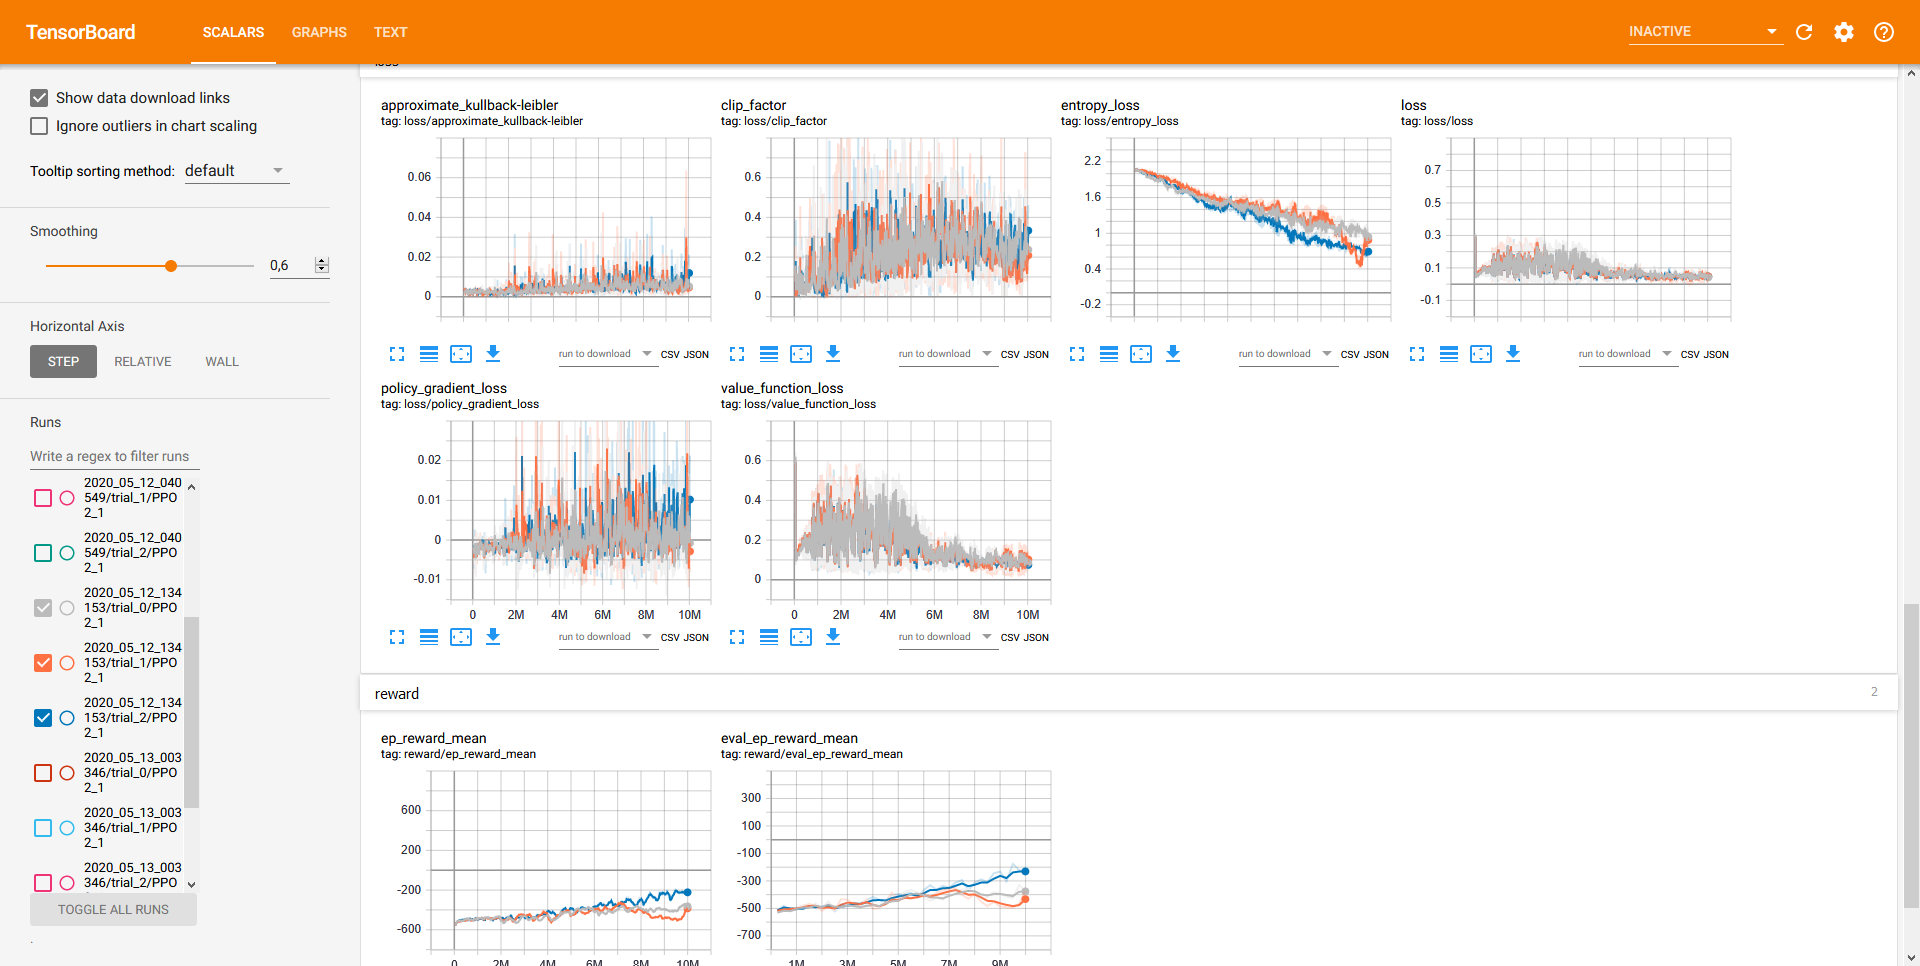
\includegraphics[clip, width=0.95\columnwidth]{figures/implementation/Tensorboard.png}
    \end{center}
    
    %\vspace*{-6pt}
    \caption[Tensorboard Example]{Example for a Tensorboard visualization.}
    \label{fig:TensorboardExample}
    %\vspace*{-12pt}
  \end{figure}

Stable Baselines already integrates Tensorboard for extended logging and visualization. Dependent on the chosen RL algorithm, Stable Baselines will log internal values like the average action advantage or the discounted reward. With Baselines Lab we extend these logging capabilities and now also include episode length and average episode reward for both training and evaluation. We also included a metric for steps per second which helps to monitor execution performance. For special modules like RND (see Section \ref{sec:blRND}) we also include module specific plots like intrinsic reward. The lab configuration is also included in the Tensorboard log file.

Tensorboard logs are created automatically at the given log directory location if the \texttt{tensorboard\_log} parameter of the algorithm is set to true.

\paragraph{Extension of Stable Baselines Functions.}
Additional to the extended monitoring, we also extended some other functions of Stable Baselines:

\begin{itemize}
    \item \textit{Learning Rate Schedules.} Stable Baselines includes an inconsistent system of learning rate schedules which are only available for a number of algorithms. In Baselines Lab we included linear and piecewise learning rate schedules for the PPO, SAC and TD3 implementations. For information on how these schedules can be used we included an example in Appendix TODO.
    \item \textit{Flexible Neural Network Creation.} Stable Baselines only allows to flexibly create dense neural networks. We extended the network base classes to also include a fully configurable network class which can be defined via config files. For an example see Appendix TODO.
\end{itemize}


\subsection{Random Network Distillation Module} \label{sec:blRND}
Since the Stable Baselines implementations do not offer any form of curiosity reward we needed to implement our own version. Huang et al. have shown, that the RND curiosity produces superior results in comparison with the original idea of an ICM module, so we decided to implement the RND reward only. 

\begin{figure}[ht]
    \begin{center}
    %\resizebox{0.95\columnwidth}{!}{%
    \begin{tabular}{c}
    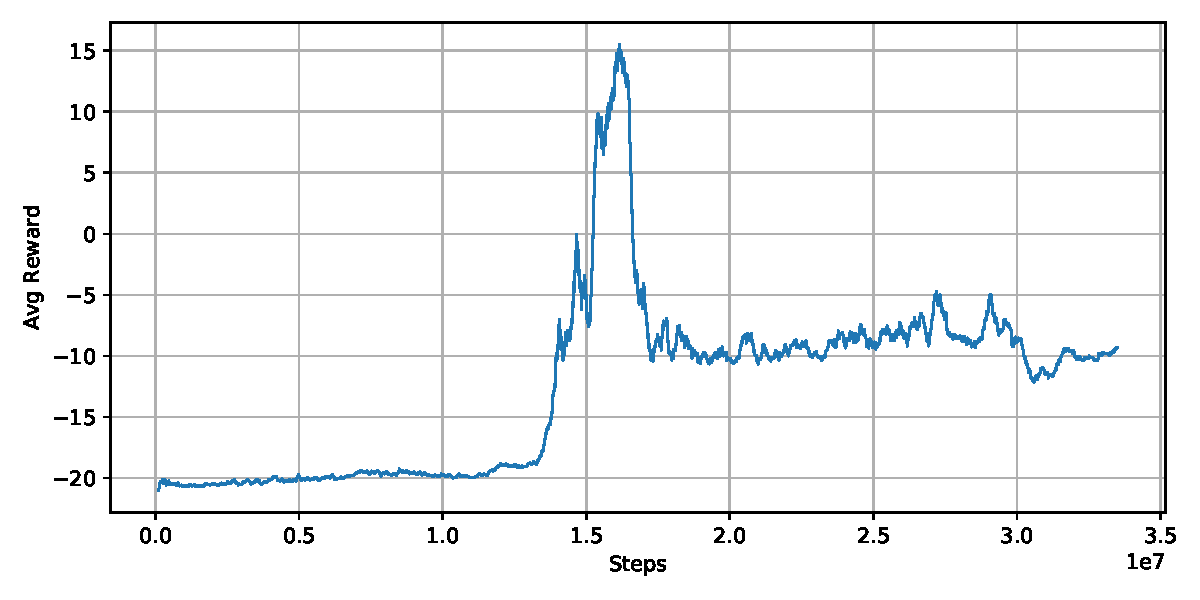
\includegraphics[clip, height=5cm]{figures/implementation/rnd_pong_episode_reward.pdf} \\
    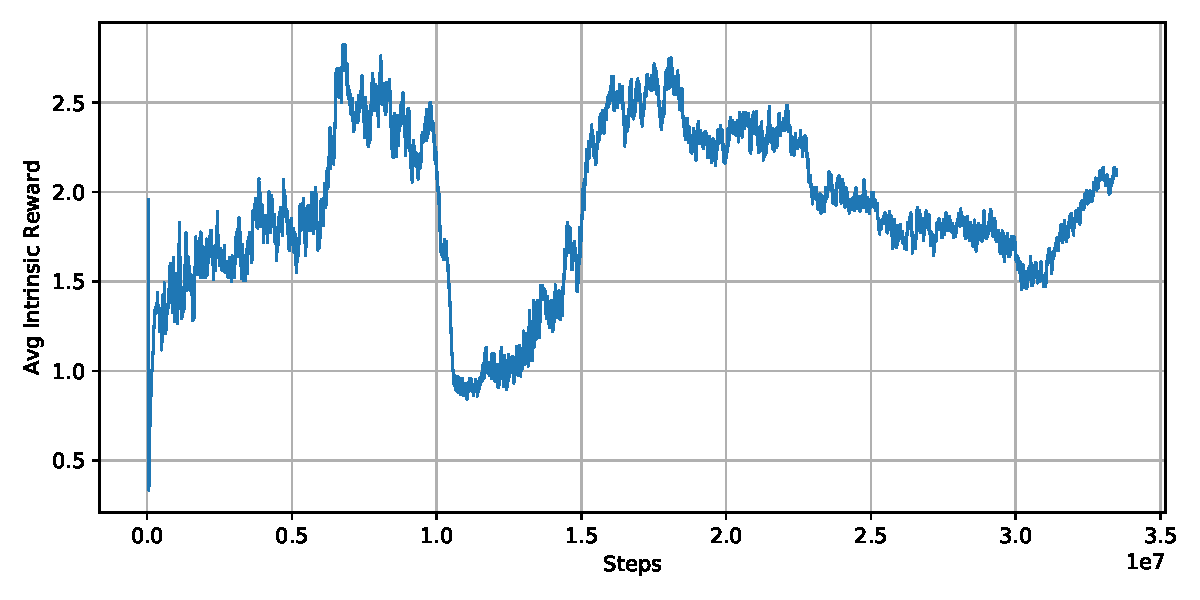
\includegraphics[clip, height=5cm]{figures/implementation/rnd_pong_episode_intrinsic_reward.pdf} \\
    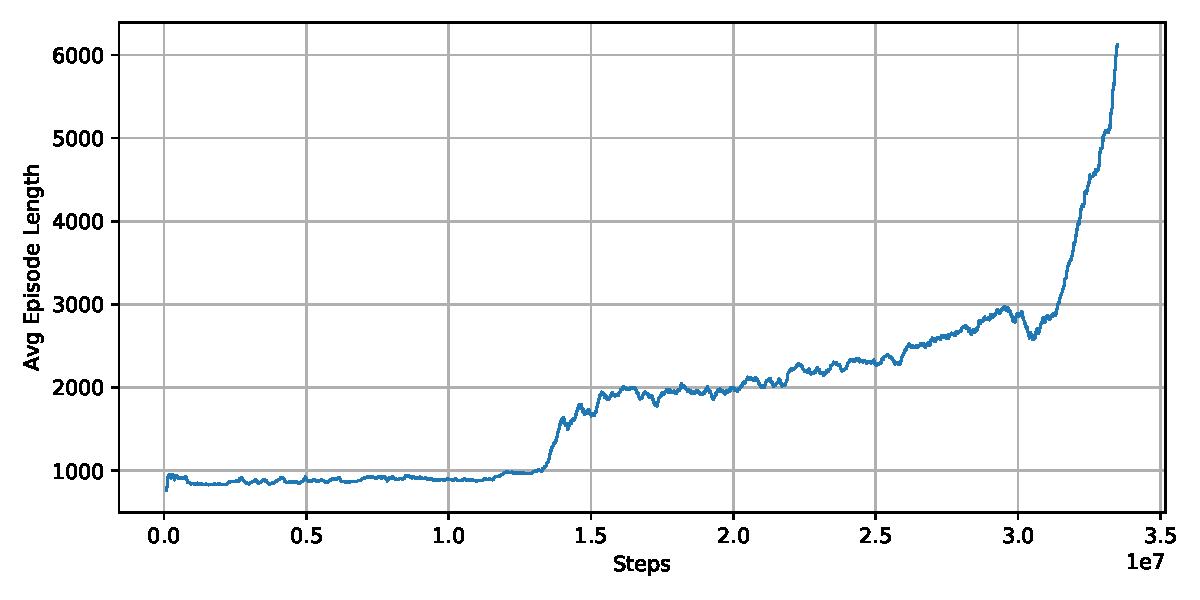
\includegraphics[clip, height=5cm]{figures/implementation/rnd_pong_episode_length.pdf} \\
    
    \end{tabular}
    %}%
    \end{center}
    %\vspace*{-12pt}
    \caption[RND on Pong]{Learning curves for the verification experiment of the curiosity reward wrapper on the Atari game Pong.}
    \label{fig:RNDPong}
    %\vspace*{-12pt}
  \end{figure}


Instead of implementing the curiosity reward as an extension of PPO (like in the original implementation) we decided to implement RND as a wrapper for the environment. This wrapper contains an internal replay buffer from which we randomly draw samples to train the predictor network. As default, we train the predictor network with the same frequency as the actor network. The replay buffer contains samples from the past four training periods. As an example, if we train 256 steps on 16 environments between each training period of the actor, the replay buffer will have a size of $256 \times 16 \times 4$ samples. We also perform four optimization epochs per training step. The networks used for the target and predictor network have the same structure as in the original implementation. 

The implementation of the RND module as a wrapper allows us to use the curiosity reward signal independent of the RL algorithm. We verified our implementation by training an PPO agent to play the Atari game "Pong" using curiosity reward only and no end-of-episode signal. Figure \ref{fig:RNDPong} shows the learning curves for intrinsic and extrinsic reward, as well as the episode length. We can see, that the agent does not optimize for extrinsic reward - this is expected, since we removed that reward signal - and instead continuously improves the intrinsic reward by increasing the episode length. The agent therefore learns to play with its enemy in Pong instead of against him. This behavior was also observed by Burda et al.\cite{burda2018exploration}.

The development of the curiosity wrapper was done in conjunction with the development team of Stable Baselines, and the implementation has been staged for a future release of Stable Baselines 3 \cite{stable-baselines-intrinsic}.

\subsection{Automated Hyperparametersearch} \label{sec:blSearch}
The choice of optimal hyperparameters is very important in any machine learning setting. As we saw in Chapter \ref{chp: RLOverview}, most RL algorithms introduce multiple new parameters, with some of them having great influence on the training performance. These parameter must be tune additional to the already existing hyperparameters like the learning rate or other optimizer specific values, an observation preprocessing pipeline and eventual environment parameters (e.g. for reward generation). Tuning all these parameters together is especially hard when because every training run may take hours before we can determine if the current configuration is better or worse than any other configuration. To support our decisions when tuning these parameters, we therefore need the possibility of an automated hyperparametersearch. 

\begin{figure}[ht]
    \lstinputlisting[language=yaml]{figures/implementation/simple_search_config.yml}
    \caption{Basic search lab configuration file.}
    \label{fig:BasicSearchConfig}
\end{figure}

To efficiently search for hyperparameters in an ML context, a number of algorithms have been developed in the past. Modern optimizer frameworks often allow to choose between a number of different of these algorithms. For Baselines Lab we choose to integrate Optuna \cite{akiba2019optuna} as it combines a number of up-to-date algorithms with great configurability. In Optuna there are mainly two classes of important algorithms: Samplers and Pruners. Samplers are used to choose from a set of hyperparameters and pruners are used to decide which trial should be canceled early (pruned). While both classes can be used with simple algorithms (e.g. a random value sampler with a median pruner), in Optuna we also can choose from more advanced algorithms. For example sampling can be done using the tree-structured parzen estimator algorithm \cite{bergstra2011algorithms} or pruning can be done via successive halving \cite{karnin2013almost} which both showed to improve performance.

In Baselines Lab it is easy to configure which sampler or pruner to use and which parameters should be tuned. In Figure \ref{fig:BasicSearchConfig} we included an example lab configuration to demonstrate how hyperparametersearch works. The shown section for the \textit{search} keyword can be appended to the lab configuration from Figure \ref{fig:BasicLabConfig} and is only used if the file is started with the \texttt{search} lab mode. We can see that we can define how many trials should be run via the \texttt{n\_trials} keyword and that we can define a sampler and a pruner method. Each pruner can receive its individual parameters by specifying them under the \texttt{pruner} keyword. For example the \textit{halving} pruner get configured such that each trial will run for at least 4000 timesteps before it can be pruned.

Depending on the chosen RL algorithm, Baselines Lab comes with a predefined set of parameter ranges which will automatically be sampled. Any parameter defined in the normal algorithm or env section will not be sampled during the parametersearch. If we want to explicitly give a range for parameters, we can redefine them under search/algorithm or search/env with a sample method and the according choices. More details can be found in the Optuna documentation \cite{optuna-docs} and in Appendix TODO.

\subsection{Additional Features} \label{sec:blAdvanced}
Baselines Lab offers a bunch of additional functions which are designed to help monitoring the training process, find problems with the learning algorithm and help with result presentation:

\begin{itemize}
    \item \textit{Plots.} Baselines Lab can automatically create plots of the tensorboard training data. To create the plots either specify \texttt{plot: true} under the \texttt{meta} keyword or use the \texttt{-{}-plot} command line argument in enjoy mode. The default plots contain train and evaluation data for reward and episode length, but it is possible to plot additional data by specifying their tensorboard tags. For more information see Appendix TODO.
    \item \textit{Video Creation.} Baselines Lab can automatically create videos of  the environment. The environment can either be rendered like it is displayed in enjoy mode (rendered for human eyes) or the environment can render the observations which are created for the agent. Both options are only available in enjoy mode and can be enabled with the command line arguments \texttt{-{}-video} or \texttt{-{}-obs-video} respectively.
    \item \textit{Email Notification.} Baselines Lab can automatically send email notifications to send updates about the training progress. This feature is only available on Linux and requires \textit{mailx} to be installed. To send email notifications we have to specify a mail address via the \texttt{-{}-mail} command line argument. 
\end{itemize}

\section{The Particle Maze Environment} \label{sec:MazeEnvironment}
Since most RL algorithms require millions of steps of training before they can solve a problem, we need a very efficient implementation for our environment. At the same time we are interested in a modular design, since we want to experiment with rewards, random goal positions, random mazes (polyominos) or even different particle models. In Section \ref{sec:MazeImplementation} we present our implementation of the basic maze environment and its modular components. In the following sections we then explain in detail how these components work, beginning with Section \ref{sec:MazeReward} where we will talk about reward generation. We then talk about extensions of the original environment to bring the simulations closer to reality with the addition of physical particles or unprecise observations in Section \ref{sec:ExtendedMaze}. Finally we will talk about random instance generation in Section \ref{sec:RandomInstanceGeneration}.

\subsection{Basic Implementation} \label{sec:MazeImplementation}
We designed the implementation for the maze environment around two key ideas: First, the environment should run as fast as possible, because the agent will need to play hundreds or thousands of episodes. Designing the environment as lightweight as possible will therefore save a lot of time during training. Second, we need an environment which is configurable with our lab configuration file system in its main aspects. This means having the possibility to dynamically load instances, define rewards and even particle behavior. For the implementation we therefore decided to build the maze environment as a modular system, which allows easy configuration and extension of the existing architecture. 

Figure \ref{fig:MazeBaseDesign} shows a simplified overview of the architecture of the environments with its main component \textit{MazeBase}. The modules which can be integrated into the MazeBase class all inherit from three interfaces and therefore can be divided into three groups:

\begin{enumerate}
    \item \textit{Instance Generators.} Instance generators load or create instances. Depending on the generator, an instance can be just created once and then returned for every future episode (e.g. if we want to load a specific instance) or the instance can be randomly generated. We will talk more about random instance creating in Section \ref{sec:RandomInstanceGeneration}.
    \item \textit{Reward Generator.} Reward generators create rewards after each step and define when the episode is over. We will talk in detail about reward shaping in Section \ref{sec:MazeReward}.
    \item \textit{Step Modifiers.} Step modifiers define the behavior of the particles. This behavior might be very simple like in the original maze implementation of Huang et al. where each particle moves exactly one step into the direction given by the action, but can be more complex. We will talk about advanced particle behavior in Section \ref{sec:ExtendedMaze}. 
\end{enumerate}

\begin{figure}[ht]
    
    \begin{center}
        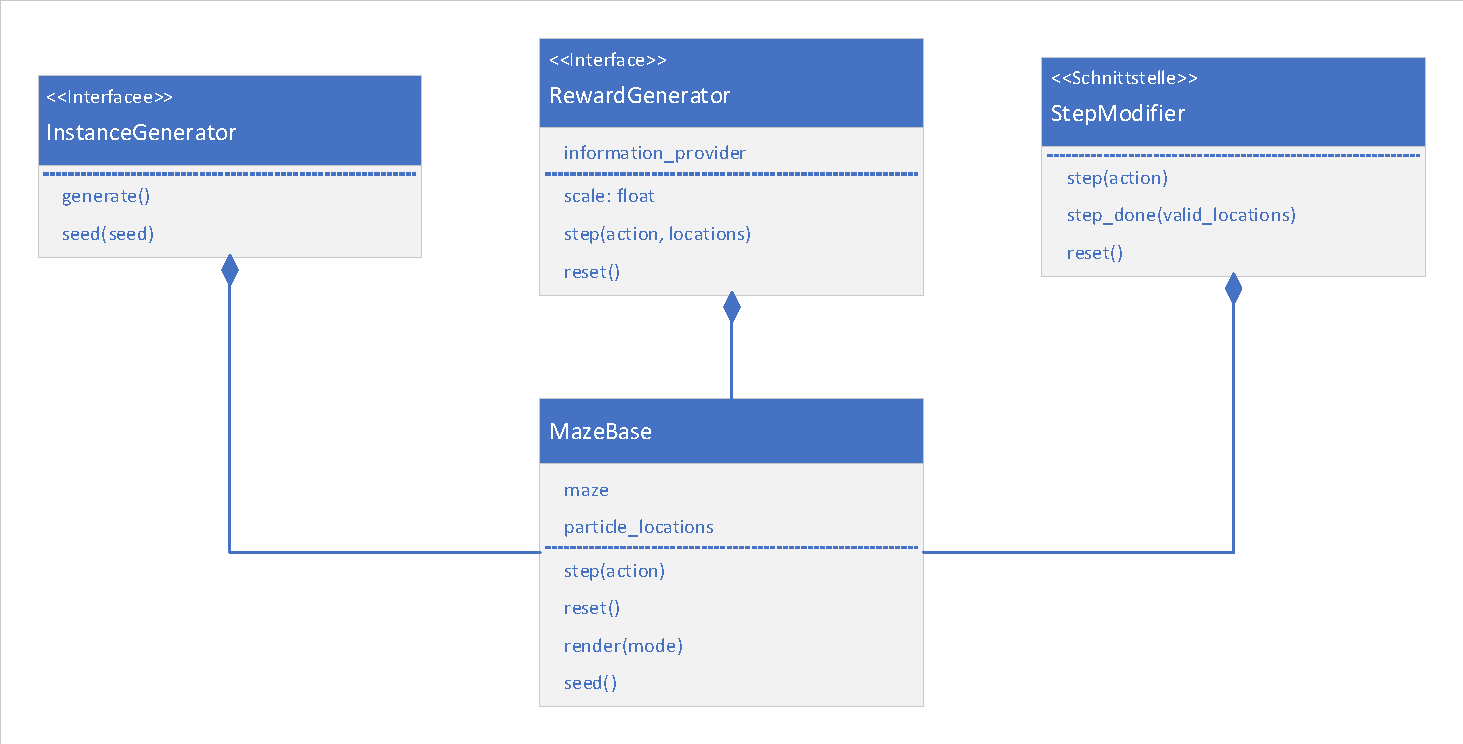
\includegraphics[clip, trim=10px 10px 10px 10px, width=0.9\columnwidth]{figures/implementation/maze_base_design.pdf}
    \end{center}
    
    %\vspace*{-6pt}
    \caption[Implementation Design for the Maze Environment]{Implementation Design for the Maze Environment.}
    \label{fig:MazeBaseDesign}
    %\vspace*{-12pt}
  \end{figure}

All components of the maze environment are generally designed with performance in mind. When implementing particle motions and reward generations, we minimized the use of python loop statements and instead solved most of the computations by utilizing NumPy \ref{oliphant2006guide} functions.

\subsection{Reward Shaping} \label{sec:MazeReward}
Rewards

\subsection{Extended Models} \label{sec:ExtendedMaze}
fuzzy, physical 

\subsection{Random Instance Generation} \label{sec:RandomInstanceGeneration}
random map generation

\section{Integration of Algorithmic Approaches} \label{sec:AlgorithmIntegration}
integration


